\documentclass[12pt,table,xcdraw]{article}
\usepackage[hidelinks]{hyperref}
\usepackage{tcolorbox}
\usepackage{moreverb}
\usepackage{geometry}
\usepackage{amsmath}
\usepackage{caption}
\usepackage{multirow}
\usepackage[table,xcdraw]{xcolor}
% \usepackage[table,xcdraw]{xcolor}
\geometry{
 a4paper,
 total={170mm,257mm},
 left=20mm,
 top=20mm,
 }
\usepackage{enumerate}
\usepackage{nopageno}
\usepackage{titlesec}
\usepackage{makecell}
\usepackage{varwidth}
\usepackage{mdframed}
\usepackage{multirow}
\usepackage{url}
\usepackage[table,xcdraw]{xcolor}
\usepackage[normalem]{ulem}
\useunder{\uline}{\ul}{}
\usepackage{longtable}
\usepackage{lscape}
\usepackage{appendix}
% \renewcommand*\thesection{\arabic{section}.0}
% \renewcommand*\thesubsection{\arabic{section}.\arabic{subsection}}
% \renewcommand*\thesubsubsection{%
%   \arabic{section}.\arabic{subsection}.\arabic{subsubsection}%
% }



\titleformat*{\section}{\fontsize{14}{14}\selectfont \bfseries}
\usepackage{graphicx}
\renewcommand{\baselinestretch}{1.25}
\pagestyle{empty}

\setcounter{secnumdepth}{5}
\begin{document}

\title{INDIAN INSTITUTE OF TECHNOLOGY TIRUPATI
  		      Chindepalle, Tirupati-517619 (AP)}

\begin{figure}[ht]
\centering

\includegraphics[width=\textwidth]{Header.png}
------------------------------------------------------------------------------------------------------------------------
\end{figure}

        \centerline{\underline{\textbf{{\fontsize{14}{16.8}\selectfont DATA SHEET}}}}


  \begin{tabbing}
      111111111111111111111111111111 \= 111111111111111 \= 1111\kill



   {\bf \large Name of the Department} \>  : \large Computer Science and Engineering\\
   {\bf 1. Name} \> : A EASHAAN RAO\\
   {\bf 2. Roll No} \> : CS21D002\\
   {\bf 3. Registration for} \> : Ph.D.\\
   {\bf 4. Specialization    } \> : Software Engineering\\
   {\bf 5. Guide(s)} \> : Dr. Sridhar Chimalakonda \\
   {\bf 6. Date of Joining} \> :  $01^{st}$ August 2019\\
   {\bf 7. Date of DC Meeting} \> : $6^{th}$ Feb 2026 \\
   {\bf 8. Area of Research } \> : Cross-Project Learning in Bug Localization

   \end{tabbing}

  \centerline{ {\bf Details of Course Work -  Ph.D.} } \vskip .1in
  {\bf Core Courses}  :\vskip .2in
  \resizebox{\textwidth}{!}{
         \begin{tabular}{|c|c|c|c|c|c|} \hline
            \textbf{S.No} & \textbf{Course No} & \textbf{Course Title}  & \textbf{Semester/Year}  & \textbf{Credit} & \textbf{Grade} \\ \hline
            1 & CS5202 & Computer System Architecture & Even/2021 & 3 & A \\ \hline

            2 & CS5208 & Distributed Systems & Even/2021 & 3 & A \\ \hline

            3 & CS5232 & Cyber Security & Even/2021 & 3 & B \\ \hline
            % 4 & ID6012 & Introduction to Research & Even 2020 & P/F & NA\\\hline
\end{tabular}}
\\
\\

    {\bf   Other Courses}  :\vskip .2in

    \begin{tabular}{|c|c|c|c|c|c|}
    \hline
    \textbf{S.No} & \textbf{Course No} & \textbf{Course Title}                                                                                                               & \textbf{Semester/Year} & \textbf{Credit} & \textbf{Grade} \\ \hline
    1             & CS6999             & \begin{tabular}[c]{@{}l@{}}Report on Critical Review\\ of Literature and Seminar \\ Presentation\end{tabular}                       & Odd/2021              & 3               & B             \\ \hline
    2             & CS7999             & \begin{tabular}[c]{@{}l@{}}Report on Simulation/\\ Preliminary/Experimental\\ /Analytical Verification \\ of Prior Art\end{tabular} & Odd/2021              & 3               & A             \\ \hline
    \end{tabular}




% {\bf Seminar Dates}  :\\
%      \centerline{NA}
%\vspace{1cm}


\vspace{4cm}
\centerline{ {\bf Details of Course Work During MS} } \vskip .1in
  {\bf Core Courses}  :\vskip .2in
  \resizebox{\textwidth}{!}{
         \begin{tabular}{|c|l|l|c|c|c|} \hline
            \textbf{S.No} & \textbf{Course No} & \textbf{Course Title}  & \textbf{Semester/Year}  & \textbf{Credit} & \textbf{Grade} \\ \hline
            1 & CS5206 & Artificial Intelligence and Machine Learning & Odd 2019 & 3 & B \\ \hline

            2 & MA5105 & Linear Algebra and Probability Theory & Odd 2019 & 4 & B \\ \hline

            3 & CS5206 & Industrial Software Engineering & Even 2020 & 3 & A \\ \hline
            4 & ID6012 & Introduction to Research & Even 2020 & P/F & P\\\hline
\end{tabular}}
\\
\\

   {\bf Elective Courses}  :\vskip .2in
   \resizebox{\textwidth}{!}{
           \begin{tabular}{|c|l|l|c|c|c|} \hline
                    \textbf{S.No} & \textbf{Course No} & \textbf{Course Title}  & \textbf{Semester/Year}  & \textbf{Credit} & \textbf{Grade} \\ \hline
                    1 & CS5101 & Advanced Data Structures and Algorithms & Odd/2019 & 3 & B \\ \hline

                    2 & CS5204 & Cloud Computing & Even 2020 & 3 & A \\  \hline
                    %3 & CS5294 & Artificial Intelligence \& Machine Learning lab & 2/1 & 2 & NA \\ \hline
                    %4 & CS5101 & Advanced Data Structures \& Algorithms lab & 1/1 & 2 & NA \\ \hline
        \end{tabular}} \\ \\ \\

\vspace{1.9cm}

\noindent
\begin{tabular}{@{}p{0.5\textwidth}@{} @{}p{0.5\textwidth}@{}}

\includegraphics[width=3cm, height=2cm]{Sridhar Sir sign.png} \hspace{9cm} 
\includegraphics[width=3cm, height=2cm]{sign.jpg}\\
\wildcard{\textbf{Signature of the Guide(s)}} & \hspace{3cm} \wildcard{\textbf{Signature of the Scholar}}
\end{tabular}

\newpage
    \begin{center}
        \underline{\textbf{{\fontsize{14}{16.8}\selectfont PROGRESS REPORT}}}
    \end{center}



\section{Thesis Introduction}
\label{sec: intro}
Bug localization (BL) is a critical software maintenance task, framed as an Information Retrieval (IR) problem. The objective is to automatically identify and rank source code files relevant to a given bug report, thereby pinpointing the likely location of the fault \cite{lam2017bug}. Majority of the existing approaches to bug localization predominantly rely on within-project models, where techniques are trained and evaluated on historical data from a single software project \cite{niu2025deep}.

Although these methods have shown improvements, their practical applicability is severely limited. They suffer from the ``cold start'' problem \cite{huo2019deep}, rendering them ineffective for new projects with no historical bug data. Furthermore, their performance is often constrained by the volume and quality of available data within a single project, a significant hurdle for smaller or less mature software systems. This performance ceiling is reflected in common evaluation metrics, even for state-of-the-art models, scores for Mean Average Precision (MAP) and Mean Reciprocal Rank (MRR) typically remain in the modest range of 0.4-0.7 \cite{niu2025deep}.

To surmount these limitations, this thesis investigates the application of cross-project learning (CPL). This paradigm involves leveraging large and diverse datasets from a multitude of ``source'' projects with the goal of training more robust and generalizable models that can effectively localize bugs in a previously unseen ``target'' project.

Prior studies exploring cross-project bug localization with Deep Learning models have shown promise \cite{huo2019deep, zhu2020cooba, liang2022modeling, zhu2022bl}, but they have not systematically evaluated or proposed effective strategies to overcome the challenge of negative transfer. The difficulty of this transition is well-documented in other research areas as well \cite{hosseini2017systematic}, stemming from significant obstacles that include vocabulary mismatch, semantic and structural incompatibilities between projects, and the aforementioned risk of ``negative transfer'', where knowledge from source projects degrades, rather than improves, performance on the target project \cite{huo2019deep}.

The central aim of this thesis is, therefore, to systematically investigate and mitigate these challenges to advance the state-of-the-art in cross-project bug localization (CPBL). This research will conduct extensive empirical investigations to develop and validate novel techniques that effectively harness the benefits of cross-project data. The primary contribution will be the creation of models that not only function reliably in a cross-project context but also outperform their within-project counterparts. The following objectives outline the planned course of this investigation.

\subsection{Objective 1: Effectiveness of Cross-Project Learning in Bug Localization Models}
\label{subsec: obj1}

The literature currently lacks a comprehensive empirical analysis that investigates the factors governing the success or failure of cross-project learning for bug localization. While the potential of CPL is acknowledged, there is little to no guidance on its practical application. Therefore, this first objective is to conduct a empirical investigation to fill this critical gap. The investigation is designed to move beyond a binary assessment of CPL's efficacy. Instead, it seeks to answer the critical questions of when, why, and how CPL is effective. Specifically, this study will:
\begin{itemize}
    \item Systematically evaluate the performance of CPL for SOTA's BL models across a diverse set of software projects.
    \item Identify and analyze the key factors (e.g., project similarity, dataset size, domain characteristics) that correlate with successful or failed knowledge transfer.
    \item Quantify the impact of negative transfer and identify the scenarios where it is most likely to occur.
\end{itemize}

The primary outcome of this objective will be a set of empirically-grounded, actionable guidelines for researchers and practitioners. These guidelines will detail how to select appropriate source projects and configure training settings to maximize the effectiveness and avoid the pitfalls of future CPL-based BL models. More discussion on objective 1 is provided in Section \ref{subsec:objecive1_plan}.

\subsection{Objective 2: A Diagnostic Study of Bug Localization in Polyglot Software Systems}
\label{subsec: obj2}
Modern software systems are polyglot in nature, utilizing multiple programming languages for implementation, configuration, and testing. Despite this, most bug localization techniques are designed and evaluated under a ``monolingual assumption'', overlooking the potential impact of task-level polyglotism, where a single bug fix spans multiple file types. This study aims to be the first empirical investigation into the architectural feasibility of SOTA bug localization models in polyglot software settings. We will evaluate both language-specific and language-agnostic models through controlled experiments on Java and Python projects from the BettleBox dataset. To enable fine-grained analysis, we introduce a bug-level categorization scheme that distinguishes between Mono-fix (single-language) and Poly-fix (multi-language) bug reports, and compare model performance across these categories. Additionally, we construct a Mono-fix-all dataset to simulate traditional ``polyglot-blind'' evaluation settings. By contrasting this with the original bug dataset, we quantify the hidden performance inflation in existing benchmarks. This study will reveal key semantic and architectural limitations in existing SOTA models, offering insights into their limited real-world applicability and highlighting new directions for future research.

\subsection{Objective 3: Novel Bug Localization Approach}
\label{subsec: obj3}
Building upon the results of the Objective 1 \& 2, the third objective is to abstract and generalize a novel approach for CPL-based bug localization. The reason is that a single, static pipeline is insufficient for the diverse software ecosystem motivates this objective; a truly robust framework must adapt to the unique characteristics of different target projects.

This objective will therefore focus on investigating and developing an adaptive mechanism. Plausible research directions include, for example, creating a set of heuristics that automatically configure the data selection strategy based on target project metadata (e.g., size, age, or domain), or designing a lightweight meta-learning model that fine-tunes the CPL pipeline for a new target project with minimal data.

The goal is to progress from a single, proof-of-concept pipeline to a reusable and configurable tool. The primary contributions of this objective will be:
\begin{itemize}
    \item The design and implementation of a generalized framework that encapsulates the core data filtering and modeling principles from the preceding objectives.
    \item A rigorous empirical validation of the framework's adaptability and effectiveness across a wide and diverse range of software projects.
    \item The delivery of a well-documented, open-source tool to enable researchers and practitioners to leverage the framework for their own bug localization needs.
\end{itemize}


\section{Work done during review}
\subsection{Objective 1: Effectiveness of Cross-Project Learning in Bug Localization Models}
\label{subsec:objecive1_plan}

The primary objective of this phase of research is to conduct a systematic and comprehensive empirical analysis of Cross-Project Learning (CPL) for the task of bug localization. The core difficulty lies in bridging the semantic gap between the natural language of bug reports and the structured nature of source code. While many methods have been developed, their performance remains suboptimal for practical use, a problem exacerbated by the scarcity of large, high-quality datasets for training robust models. CPL has emerged as a promising technique to address this by leveraging data from multiple source projects to improve performance on a target project. However, CPL introduces its own challenges, such as domain shift and vocabulary mismatch, and its effectiveness has not yet been thoroughly studied under controlled, multi-metric evaluation conditions. This study addresses that gap by not only evaluating whether CPL works, but by systematically identifying the precise conditions under which it succeeds or fails, and by empirically validating the first data-driven strategy for source project selection.

To achieve this, the study employs \textbf{TRANP-CNN} \cite{huo2019deep}, a convolutional neural network-based reranking model, as the representative SOTA bug localization model for Phase 1 evaluation. The evaluation is structured around four training scenarios designed to isolate the contribution of cross-project data at varying levels of target-project data availability. The study is guided by the following research questions:

\begin{itemize}
    \item \textbf{RQ1}: Does cross-project transfer (CP-transfer) significantly outperform within-project training on limited data (WP-small) across multiple evaluation metrics?\\
    \textbf{Motivation}: This is the core CPL feasibility question. Prior work has asserted CPL's promise but has not reported matched-budget comparisons with statistical significance testing across a large and diverse project corpus.

    \item \textbf{RQ2}: What target-project characteristics are the strongest predictors of CPL performance, and do these predictors hold consistently across retrieval and ranking metrics?\\
    \textbf{Motivation}: Understanding which project properties drive or limit performance is essential for practical deployment guidance. This question investigates whether source- or target-side features are more predictive, and whether recall and ranking metrics reveal different signals.

    \item \textbf{RQ3}: Can a data-driven heuristic reliably identify the best source project for a given target, and what is the upper bound on source selection quality?\\
    \textbf{Motivation}: No prior CPBL study has formally validated source selection strategies beyond intuitive domain-matching. This question establishes an empirical benchmark for source selection quality using Kendall rank correlation and Hit@1 accuracy.

    \item \textbf{RQ4}: Is the FAISS-based retrieval stage a limiting factor in the end-to-end CPL pipeline, or does the performance ceiling reside entirely in the reranking model?\\
    \textbf{Motivation}: Diagnosing whether failures originate in retrieval (ground-truth file not retrieved) or in reranking (file retrieved but ranked too low) directly informs where architectural investment is most valuable.
\end{itemize}

\subsubsection{Experimental Setup}

\paragraph{Dataset Selection and Curation.}
The experimental corpus comprises \textbf{20 open-source software projects} drawn from five established bug localization benchmark datasets: \textbf{Bench4BL} \cite{lee2018bench4bl}, \textbf{BeetleBox} \cite{chakraborty2025blaze}, \textbf{LCA} \cite{ciborowska2022fast}, \textbf{SWE-bench} \cite{jimenez2023swe}, and the dataset of \textbf{Ye et al.} \cite{ye2014learning}. Projects were selected to ensure diversity in programming language (Python and Java), codebase size (ranging from approximately 2,000 to 438,000 Lines of Code), application domain (scientific computing, machine learning, data visualization, web frameworks, and enterprise systems), and historical bug report volume (ranging from 23 to 1,609 unique bug reports per project). The consolidated dataset comprises \textbf{94 unique source$\rightarrow$target project pairs}, yielding \textbf{373 individual experiment runs} across four evaluation scenarios. Table~\ref{tab:dataset} summarizes selected representative projects.

\begin{table}[h]
\centering
\caption{Representative projects from the experimental corpus.}
\label{tab:dataset}
\resizebox{\textwidth}{!}{
\begin{tabular}{|l|c|c|c|c|}
\hline
\textbf{Project} & \textbf{Language} & \textbf{LoC} & \textbf{Bug Reports} & \textbf{Domain} \\ \hline
numpy/numpy & Python & 276,481 & 527 & Scientific Computing \\ \hline
jupyterlab/jupyterlab & Python & 39,372 & 197 & Dev Tools \\ \hline
matplotlib/matplotlib & Python & 248,837 & 183 & Visualization \\ \hline
scipy/scipy & Python & 438,217 & 100 & Scientific Computing \\ \hline
scikit-learn/scikit-learn & Python & 175,621 & 483 & Machine Learning \\ \hline
spring-projects/spring-data-jpa & Java & 24,810 & 375 & Web/Enterprise \\ \hline
wildfly/wildfly & Java & 312,004 & 1,609 & Application Server \\ \hline
\end{tabular}}
\end{table}

\paragraph{Dataset Preprocessing.}
The preprocessing pipeline is structured into two distinct stages. In the first stage, bug report preprocessing, raw bug reports are extracted from the respective benchmark datasets and deduplicated by commit SHA to ensure each report maps to a unique ground-truth file set. Reports with missing ground-truth annotations or malformed commit references are discarded, resulting in a clean corpus of project-level bug metadata stored in a standardized Parquet format. In the second stage, source code embedding, all source files from each project repository are chunked into segments of 512 tokens with an overlap of 50 tokens, and each chunk is encoded using the \textbf{BAAI/bge-code-v1} \cite{bge_embedding} embedding model (768-dimensional, float32). These chunk-level embeddings are averaged to produce a single file-level embedding, stored as \texttt{float32} vectors in per-project pickle files. Bug report embeddings are generated analogously by encoding the full bug report text. The resulting per-project \textit{blob embedding databases} and \textit{bug metadata databases} serve as the foundation for both retrieval and domain gap computation.

\paragraph{Evaluation Pipeline.}
The study adopts a \textbf{Retriever-Reranker} architecture. The retriever is a \textbf{FAISS IndexFlatIP} (inner-product search after L2 normalization), which retrieves the top-$K$ = 300 candidate source files for each bug report. The reranker is \textbf{TRANP-CNN} \cite{huo2019deep}, a CNN-based model that takes the (bug report, candidate file) pair as input and produces a relevance score used to re-rank the 300 candidates. This architecture decouples retrieval quality from reranking quality, enabling precise diagnosis of where failures occur.

\paragraph{Training Scenarios.}
Every source$\rightarrow$target pair is evaluated under four training regimes, as described in Table~\ref{tab:scenarios}.

\begin{table}[h]
\centering
\caption{Four evaluation scenarios and their data configurations.}
\label{tab:scenarios}
\begin{tabular}{|l|l|p{6.5cm}|}
\hline
\textbf{Scenario} & \textbf{Training Data} & \textbf{Research Relevance} \\ \hline
WP-small & 20\% target bugs only & Baseline: limited within-project training \\ \hline
WP-large & 80\% target bugs only & Upper bound: maximum within-project training \\ \hline
CP-cold-start & 100\% source, 0\% target & Zero-shot cross-project transfer \\ \hline
CP-transfer & 100\% source + 20\% target & Core CPL hypothesis: cross-project pre-training with minimal target fine-tuning \\ \hline
\end{tabular}
\end{table}

\paragraph{Evaluation Metrics.}
Five complementary metrics are reported throughout this study to provide a complete picture of both retrieval and ranking performance. \textbf{Top-$K$ Recall} ($K \in \{1, 5, 10\}$) measures the fraction of bug reports for which the ground-truth file appears within the top $K$ ranked candidates. \textbf{Mean Average Precision (MAP)} measures the average precision at each rank position where a relevant file appears, rewarding models that place correct files higher in the ranking. \textbf{Mean Reciprocal Rank (MRR)} computes the mean of $1/\text{rank}$ across all bug reports, where rank is the position of the first correct answer. Together, Top-$K$ captures retrieval breadth while MAP and MRR capture ranking precision. It is important to note that these two families of metrics can diverge: a model may achieve high Top-10 recall but low MRR if the correct file is consistently ranked at position 9 rather than 1. Both perspectives are reported to avoid misleading conclusions.

\paragraph{Domain Gap Measurement.}
To quantify the structural dissimilarity between project pairs, a \textbf{domain gap} score is computed for each source$\rightarrow$target combination by training a \texttt{LogisticRegression} binary classifier on the blob embeddings of the two projects. The resulting classification accuracy serves as the domain gap metric: a score closer to 1.0 indicates that the two projects occupy largely disjoint regions of the embedding space, while a score closer to 0.5 indicates significant overlap.

\subsubsection{Results and Discussion}

\paragraph{Overall Scenario Performance (RQ1).}
Table~\ref{tab:overall} presents the mean performance across all 92--94 source$\rightarrow$target pairs for each evaluation scenario. A consistent ordering is observed across all five metrics: WP-large $>$ CP-transfer $>$ WP-small $>$ CP-cold-start. CP-transfer, which uses the same 20\% target data budget as WP-small but augments it with 100\% source project pre-training, consistently outperforms WP-small while approaching WP-large.

\begin{table}[h]
\centering
\caption{Mean performance across all pairs for each scenario.}
\label{tab:overall}
\begin{tabular}{|l|c|c|c|c|c|}
\hline
\textbf{Scenario} & \textbf{Top-1} & \textbf{Top-5} & \textbf{Top-10} & \textbf{MAP} & \textbf{MRR} \\ \hline
WP-large      & 0.081 & 0.200 & 0.258 & 0.218 & 0.248 \\ \hline
CP-transfer   & 0.064 & 0.189 & 0.251 & 0.197 & 0.226 \\ \hline
WP-small      & 0.056 & 0.167 & 0.223 & 0.176 & 0.202 \\ \hline
CP-cold-start & 0.005 & 0.021 & 0.040 & 0.038 & 0.042 \\ \hline
\end{tabular}
\end{table}

To assess whether the advantage of CP-transfer over WP-small is statistically reliable, a \textbf{Wilcoxon signed-rank test} is applied to each metric. This non-parametric paired test is appropriate because: (i) the observations are paired---each source$\rightarrow$target pair contributes one CP-transfer and one WP-small result---and (ii) the distributions of improvements cannot be assumed normal across such a diverse project corpus. The one-sided alternative is tested (CP-transfer $>$ WP-small). Results are reported in Table~\ref{tab:wilcoxon}.

\begin{table}[h]
\centering
\caption{Wilcoxon signed-rank test: CP-transfer vs. WP-small (one-sided, $H_1$: CP-transfer $>$ WP-small).}
\label{tab:wilcoxon}
\begin{tabular}{|l|c|c|c|}
\hline
\textbf{Metric} & \textbf{Win Rate} & \textbf{Mean Gain} & \textbf{$p$-value} \\ \hline
Top-1  & 37.0\% & +0.007 & 0.118 (n.s.) \\ \hline
Top-5  & 43.5\% & +0.021 & 0.007 ($\star\star$) \\ \hline
Top-10 & 47.8\% & +0.026 & 0.001 ($\star\star$) \\ \hline
MAP    & 64.1\% & +0.020 & 0.006 ($\star\star$) \\ \hline
MRR    & 67.4\% & +0.022 & 0.005 ($\star\star$) \\ \hline
\end{tabular}
\end{table}

The results demonstrate that CP-transfer produces statistically significant improvements over WP-small for MAP, MRR, Top-5, and Top-10 ($p < 0.01$), while Top-1 improvement is not statistically significant ($p = 0.118$). This finding reveals an important nuance: CPL's advantage is primarily in \textit{ranking quality}---the model learns to order candidate files more accurately from cross-project training---but does not consistently elevate the correct file to the very top position. Comparing CP-transfer against WP-large, the gap narrows considerably on recall metrics: CP-transfer matches or exceeds WP-large on Top-10 in 53.3\% of pairs and comes within 10\% in 63.0\% of pairs. The gap is more pronounced for MAP (CP-transfer $\geq$ WP-large in only 30.4\% of pairs) and MRR (32.6\%), indicating that WP-large retains a ranking precision advantage that CPL does not fully close with the current architecture.

\paragraph{Target Properties as Performance Predictors (RQ2).}
To identify the features most predictive of CPL performance, \textbf{Spearman rank correlation} is computed between project-level metadata features and CP-transfer performance for each metric. Spearman's $\rho$ is used rather than Pearson's because the project corpus spans several orders of magnitude in codebase size and bug count, making a linear association assumption inappropriate. A Spearman correlation of $\rho = +1.0$ indicates a perfect positive monotonic relationship, $\rho = -1.0$ a perfect negative monotonic relationship, and $\rho = 0$ indicates the absence of a systematic association. Results are reported in Table~\ref{tab:spearman}.

\begin{table}[h]
\centering
\caption{Spearman rank correlations ($\rho$) between project features and CP-transfer performance. Statistical significance: $\star\star\star$ ($p < 0.001$), $\star\star$ ($p < 0.01$), $\star$ ($p < 0.05$), n.s. (not significant).}
\label{tab:spearman}
\begin{tabular}{|l|c|c|c|c|}
\hline
\textbf{Feature} & \textbf{Top-10 $\rho$} & \textbf{MAP $\rho$} & \textbf{MRR $\rho$} & \textbf{Sig.} \\ \hline
Target LoC (tgt\_LoC)               & $-0.855$ & $-0.652$ & $-0.667$ & $\star\star\star$ \\ \hline
Target bug verbosity                & $+0.333$ & $+0.383$ & $+0.297$ & $\star\star\star / \star\star$ \\ \hline
Target bug count (tgt\_n\_bugs)     & $+0.134$ & $+0.311$ & $+0.319$ & n.s. / $\star\star$ \\ \hline
Source LoC (src\_LoC)               & $+0.274$ & $+0.252$ & $+0.259$ & $\star\star / \star$ \\ \hline
Source bug count (src\_n\_bugs)     & $-0.045$ & $+0.016$ & $+0.070$ & n.s. \\ \hline
Domain gap                          & $+0.116$ & $+0.012$ & $+0.038$ & n.s. \\ \hline
\end{tabular}
\end{table}

The most striking finding is that \textbf{target codebase size (tgt\_LoC) is by far the strongest predictor}, with $\rho = -0.855$ for Top-10 recall---a very strong negative correlation that is consistent across all five metrics. This indicates that as the target project's codebase grows, the correct source file is increasingly buried within a large candidate pool, making precise ranking progressively harder regardless of the source project used. The second-most important feature is target bug report verbosity ($\rho = +0.383$ for MAP), which captures the descriptive richness of bug descriptions; more detailed reports provide stronger textual matching signals for the embedding model. Critically, \textbf{source-side features are weak or non-significant}: source bug count ($\rho = 0.07$ for MRR, n.s.) and domain gap ($\rho = 0.038$ for MRR, n.s.) show no reliable predictive power. This finding directly challenges the intuitive assumption that source-target similarity is the primary driver of CPL success, and shifts the focus to target-project viability as the dominant factor.

Furthermore, the CPL gain (defined as CP-transfer$-$WP-small MRR) is \textbf{3--4$\times$ larger for data-scarce targets}: for targets with $\leq 228$ bug reports (the median), the mean Top-10 gain is $+0.043$, compared to $+0.007$ for targets with more than 228 reports. This result positions CPL as most valuable precisely where it is most needed---for new, small, or low-activity projects with insufficient within-project training data.

\paragraph{Source Project Selection (RQ3).}
To formally evaluate the feasibility of data-driven source project selection, \textbf{Kendall's rank correlation ($\tau$)} is computed between the ordering produced by candidate selection strategies and the oracle ordering (sorted by actual achieved CP-transfer MRR) for each of the 12 target projects with at least three available source candidates. Kendall's $\tau$ ranges from $-1$ (perfectly reversed ordering) to $+1$ (perfectly aligned ordering), with $\tau = 0$ indicating no systematic relationship between the heuristic and oracle rankings. Additionally, \textbf{Hit@1 accuracy} is reported: the fraction of targets for which the strategy selects the oracle-best source.

The \textbf{most-bugs heuristic}---selecting the source project with the largest bug corpus---achieves a Hit@1 of \textbf{41.7\%} (5 out of 12 targets) and a mean Kendall $\tau$ of \textbf{$+0.253$}. Table~\ref{tab:source_selection} compares strategies against the oracle upper bound and a random baseline.

\begin{table}[h]
\centering
\caption{Source selection strategy comparison across 12 targets ($\geq$ 3 source candidates).}
\label{tab:source_selection}
\begin{tabular}{|l|c|c|c|c|}
\hline
\textbf{Strategy} & \textbf{Mean MRR} & \textbf{Mean MAP} & \textbf{Hit@1} & \textbf{Mean $\tau$ (MRR)} \\ \hline
Oracle (upper bound) & 0.320 & 0.273 & 100\% & --- \\ \hline
Most-bugs heuristic  & 0.293 & 0.249 & 41.7\% & $+0.253$ \\ \hline
Random (lower bound) & 0.262 & 0.228 & $\sim$15\% & $\sim$0.00 \\ \hline
\end{tabular}
\end{table}

The most-bugs heuristic captures approximately 53\% of the gap between random and oracle selection ($(0.293 - 0.262) / (0.320 - 0.262) = 0.53$). Importantly, the domain gap and bug report similarity---both intuitively appealing proxies for source-target relevance---show no significant correlation with achieved CP-transfer performance ($\rho < 0.12$, $p > 0.05$ for all metrics). These findings establish that while a useful heuristic exists, source project selection remains a \textbf{partially solved problem}: the heuristic fails in 58\% of cases, and a learned meta-model capable of generalizing to unseen targets represents a clear direction for future work.

\paragraph{FAISS Retrieval Ceiling (RQ4).}
Across all 94 source$\rightarrow$target pairs and all four scenarios, the fraction of bug reports for which the ground-truth file is absent from the FAISS top-300 candidates---denoted \textbf{pct\_unreachable}---is \textbf{0.00\%}. This finding has a critical architectural implication: every failure in the end-to-end pipeline is a \textit{reranking failure}, not a retrieval failure. The BAAI/bge-code-v1 embeddings are sufficiently expressive to retrieve the correct file within 300 candidates in all cases. The performance bottleneck lies entirely in TRANP-CNN's ability to promote that file from its initial FAISS rank (which can be as high as rank 167 for large-codebase targets) to within the top-10. Increasing the retrieval pool beyond $K = 300$ is therefore unlikely to yield meaningful improvements; instead, architectural advances in the reranker---such as replacing the CNN with a transformer-based or graph neural network-based model---represent the highest-impact research direction.

\paragraph{Showcase Analysis: Three Illustrative Pairs.}
To move beyond aggregate statistics and illustrate the range of CPL behaviours observed, three representative source$\rightarrow$target pairs are selected for in-depth analysis.

\textbf{Pair B: numpy $\rightarrow$ jupyterlab (Best CPL Performer).} This pair illustrates the strongest CPL performance in the corpus. Table~\ref{tab:pair_b} reports all five metrics across the four scenarios for the primary direction (numpy as source, jupyterlab as target).

\begin{table}[h]
\centering
\caption{Pair B (numpy $\rightarrow$ jupyterlab): per-scenario performance. jupyterlab: 39K LoC, 197 bug reports.}
\label{tab:pair_b}
\begin{tabular}{|l|c|c|c|c|}
\hline
\textbf{Scenario} & \textbf{Top-5} & \textbf{Top-10} & \textbf{MAP} & \textbf{MRR} \\ \hline
WP-large      & 1.000 & 1.000 & --- & 0.724 \\ \hline
CP-transfer   & 1.000 & 1.000 & --- & 0.666 \\ \hline
WP-small      & 0.870 & 1.000 & --- & 0.464 \\ \hline
CP-cold-start & 0.348 & 0.565 & --- & 0.258 \\ \hline
FAISS baseline & --- & --- & --- & 0.022 \\ \hline
\end{tabular}
\end{table}

CP-transfer (MRR = 0.666) closely approaches WP-large (MRR = 0.724) while using the same 20\% target data as WP-small (MRR = 0.464). Top-5 and Top-10 recall reach 100\% for both CP-transfer and WP-large, meaning every jupyterlab bug report is localized within the top-10 files. The FAISS baseline MRR of 0.022 underscores the magnitude of the reranker's contribution: a 33$\times$ improvement over raw embedding retrieval.

\begin{figure}[h]
\centering
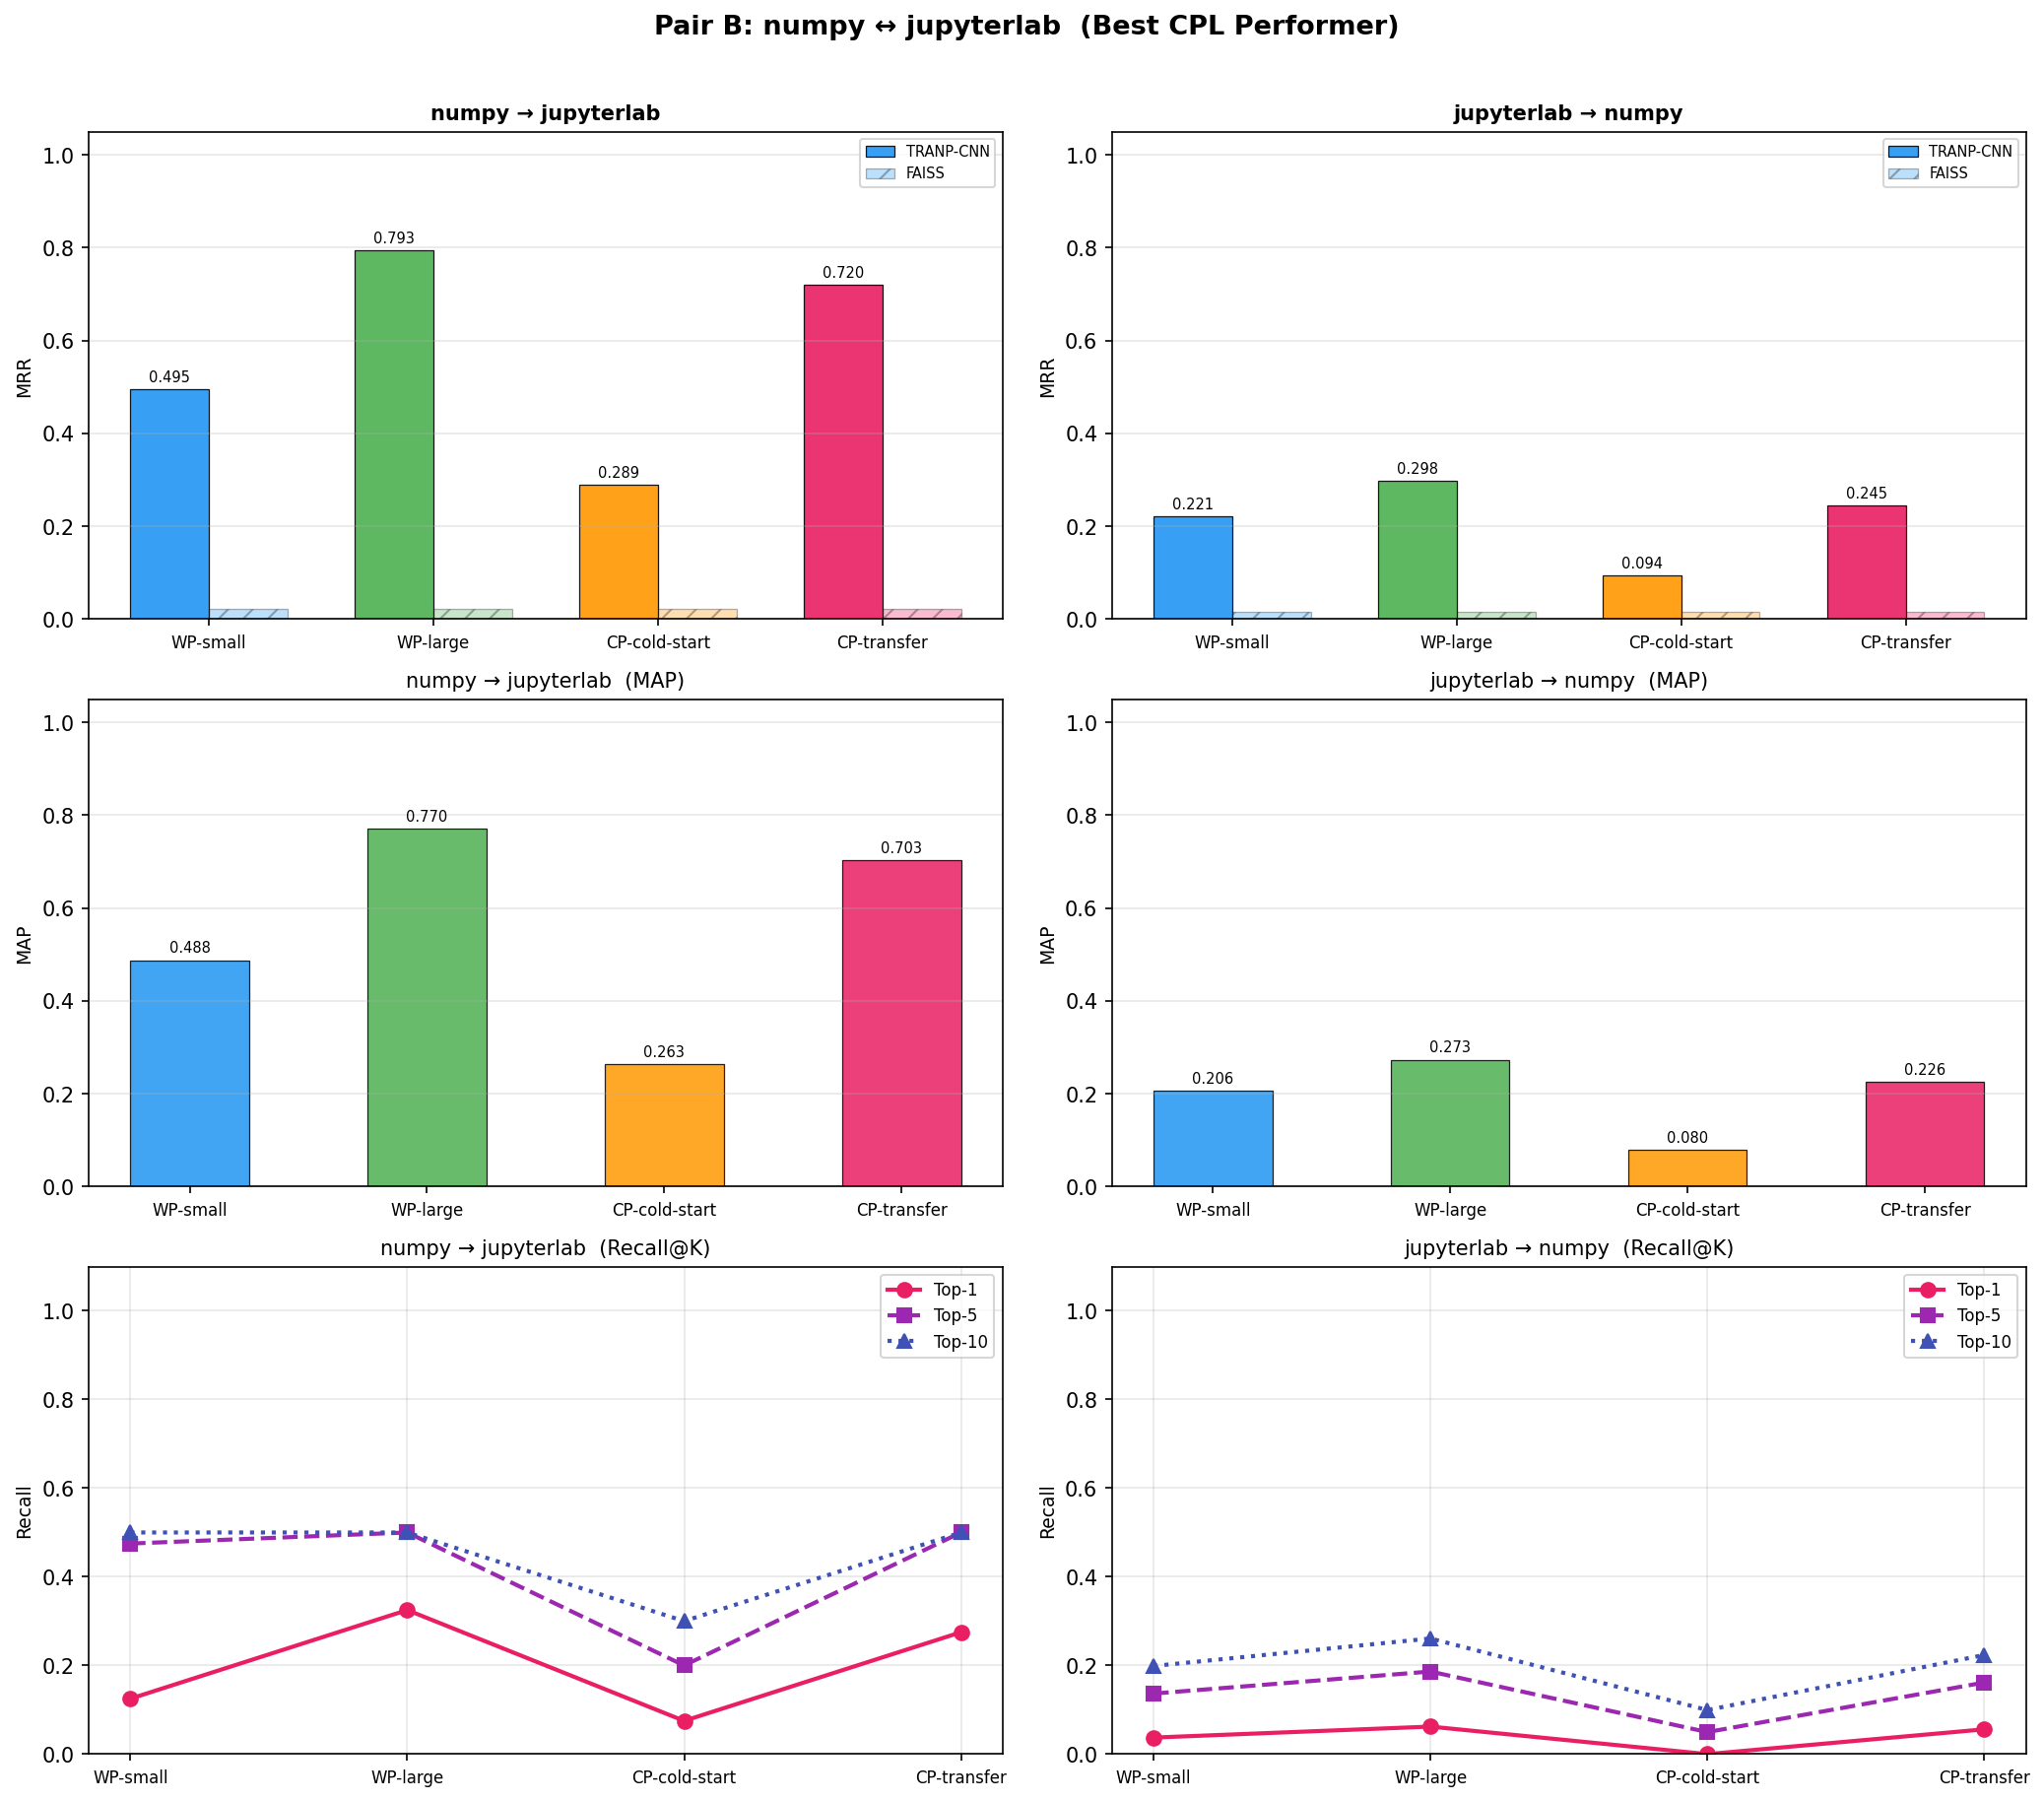
\includegraphics[width=\textwidth]{all_metrics_comparison.png}
\caption{Pair B (numpy $\leftrightarrow$ jupyterlab): all five metrics across four scenarios for both transfer directions. Top row: MRR with FAISS baseline overlay. Middle row: MAP. Bottom row: Top-K recall curves.}
\label{fig:pair_b}
\end{figure}

Figure~\ref{fig:pair_b} presents the full metric breakdown for both directions of this pair. The forward direction (numpy $\rightarrow$ jupyterlab, left column) shows strong and consistent improvements across all scenarios. The reverse direction (jupyterlab $\rightarrow$ numpy) shows substantially lower performance, consistent with the commutativity analysis discussed below.

\textbf{Pair A: matplotlib $\leftrightarrow$ jupyterlab (Commutativity Contrast).} This pair illustrates the most pronounced commutativity asymmetry in the corpus. The two projects share an identical domain gap score of 0.972 (high dissimilarity), yet the CPL outcome reverses entirely when the source and target roles are swapped.

\begin{table}[h]
\centering
\caption{Pair A: asymmetric CPL performance across transfer directions (MRR).}
\label{tab:pair_a}
\begin{tabular}{|l|c|c|c|c|}
\hline
\textbf{Direction} & \textbf{WP-small} & \textbf{WP-large} & \textbf{CP-cold-start} & \textbf{CP-transfer} \\ \hline
matplotlib $\rightarrow$ jupyterlab & 0.438 & 0.554 & 0.045 & \textbf{0.614} \\ \hline
jupyterlab $\rightarrow$ matplotlib & 0.372 & 0.294 & 0.320 & 0.236 \\ \hline
\end{tabular}
\end{table}

In the forward direction, where jupyterlab (39K LoC) serves as the target, CP-transfer (0.614) is the strongest scenario and outperforms WP-large (0.554). In the reverse direction, where matplotlib (249K LoC) serves as the target, CP-transfer (0.236) is the weakest scenario and falls below WP-small (0.372). This reversal is entirely attributable to target codebase size, consistent with the dominant Spearman correlation of $\rho = -0.855$ for tgt\_LoC. Figure~\ref{fig:pair_a_comm} visualizes the commutativity asymmetry across both MRR and MAP, further confirming that this is not an artefact of a single metric.

\begin{figure}[h]
\centering
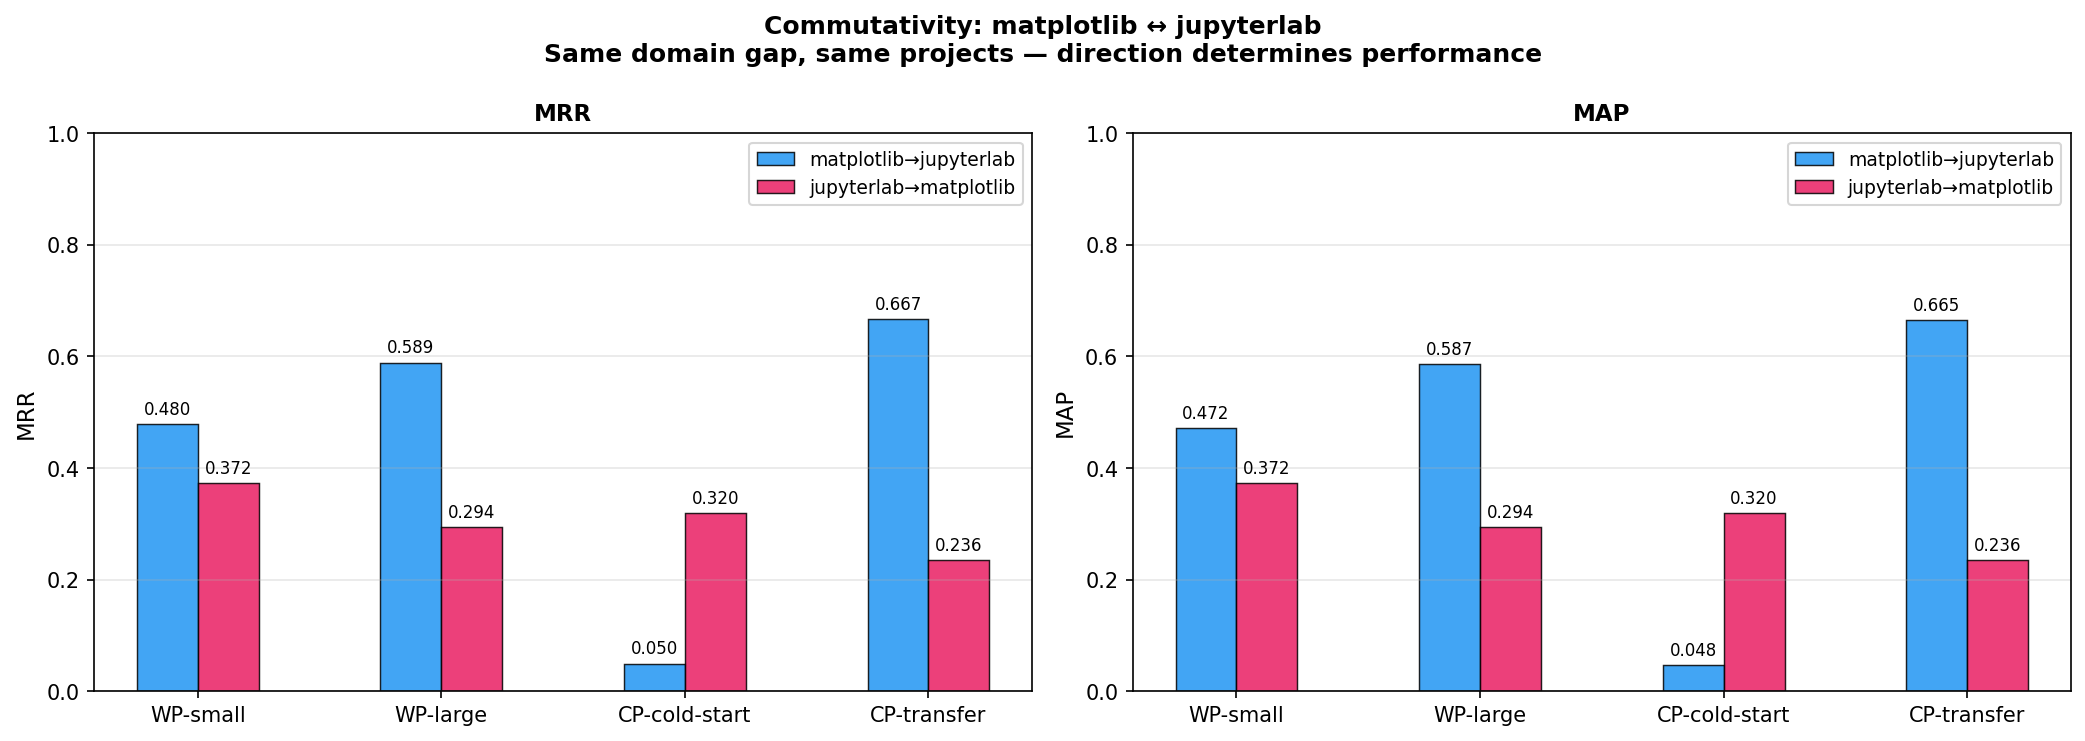
\includegraphics[width=\textwidth]{commutativity_contrast.png}
\caption{Pair A (matplotlib $\leftrightarrow$ jupyterlab): commutativity contrast for MRR (left) and MAP (right). The same domain gap (0.972) and same project pair produce opposite CPL outcomes depending on which project is the target, driven entirely by target codebase size.}
\label{fig:pair_a_comm}
\end{figure}

\textbf{Pair C: numpy $\rightarrow$ scipy (Hard Target Ceiling).} scipy (438K LoC, 100 bug reports) represents the extreme large-codebase scenario. All four scenarios yield Top-1, Top-5, and Top-10 recall of 0.00, with MRR peaking at 0.029 for WP-large. Despite this, pct\_unreachable = 0\%: the ground-truth file is present in the FAISS top-300 for every bug report. Figure~\ref{fig:pair_c_disp} displays the rank displacement distributions across scenarios, confirming that the reranker does improve rankings (mean displacement $= +131$ for WP-large) but cannot overcome the scale of the search space. This pair illustrates the target viability threshold: when the target codebase exceeds $\approx$200K LoC, no source project can compensate for the architectural limitation of the current reranker.

\begin{figure}[h]
\centering
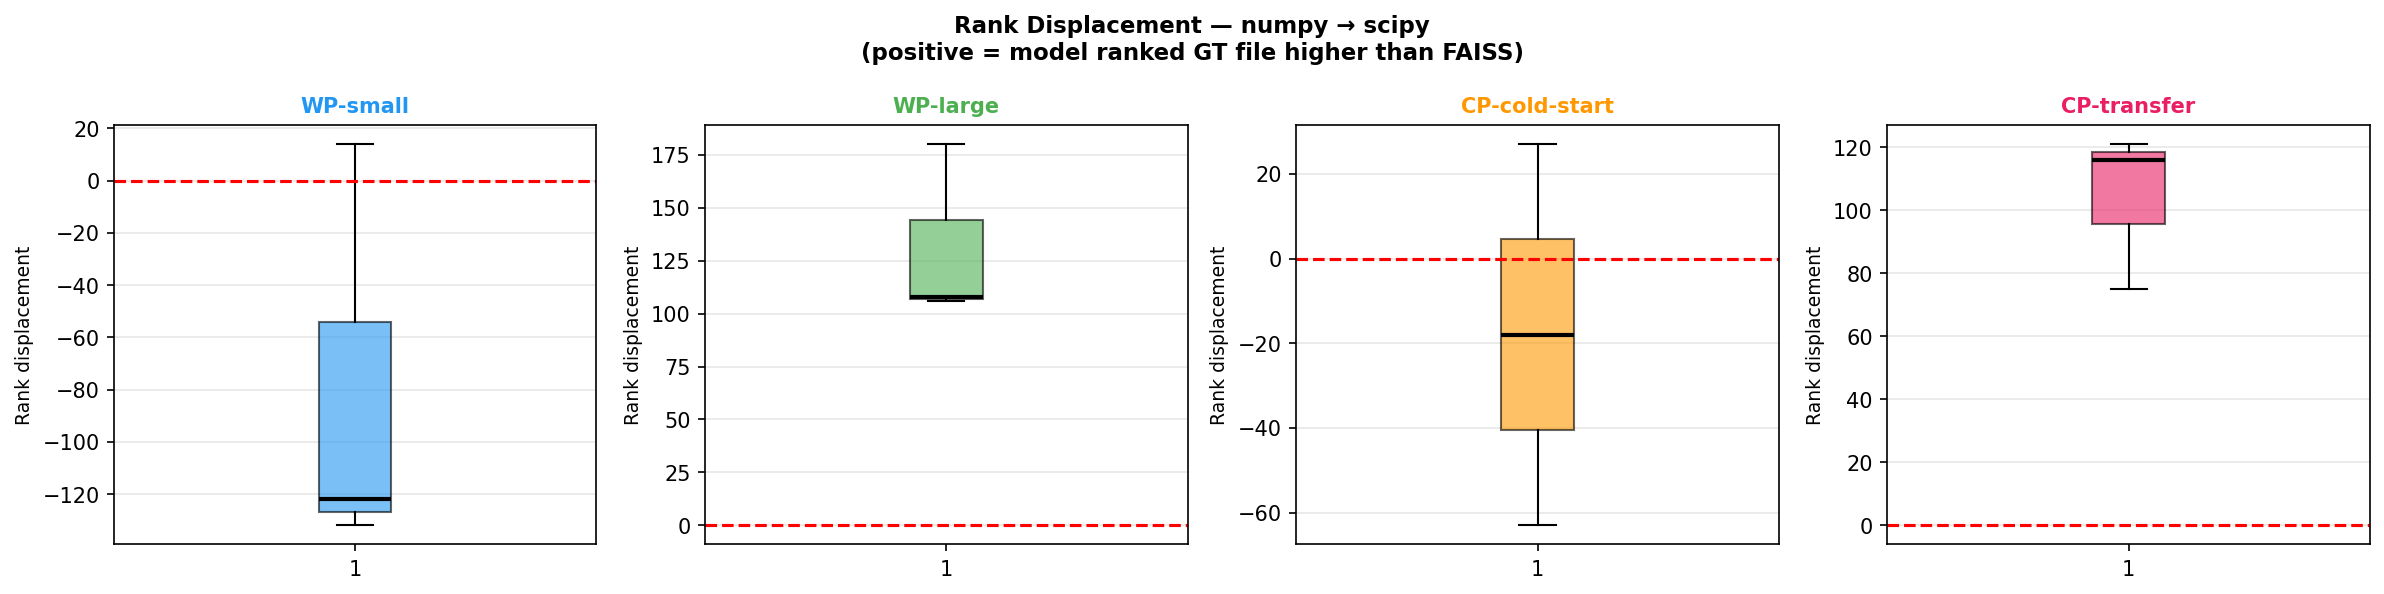
\includegraphics[width=\textwidth]{rank_displacement_boxplot.png}
\caption{Pair C (numpy $\rightarrow$ scipy): rank displacement distributions per scenario. Positive displacement indicates the model improved the GT file's rank relative to FAISS. The model does improve ranks substantially (WP-large median $>$ 0), but the improvement is insufficient to break into the top-10 given scipy's 438K LoC search space.}
\label{fig:pair_c_disp}
\end{figure}

\subsubsection{Limitations}

This study is subject to several limitations that should be considered when interpreting the findings and applying the resulting guidelines.

\textbf{Single model evaluated in Phase 1.} The Phase 1 analysis is conducted exclusively with TRANP-CNN \cite{huo2019deep}. While this provides a controlled and internally consistent evaluation, the conclusions---particularly regarding the magnitude of CPL gain and the ranking precision gap relative to WP-large---may not generalize uniformly to other SOTA architectures such as FLIM \cite{liang2022modeling}, BL-GAN \cite{zhu2022bl}, or COOBA \cite{zhu2020cooba}, which differ in their reliance on structural code features (e.g., AST-based representations) and training objectives.

\textbf{Programming language coverage.} The current experimental corpus is predominantly Python-based, with a subset of Java projects. The generalizability of the Spearman correlations---particularly the dominant effect of tgt\_LoC---to C++, JavaScript, or polyglot projects remains empirically unvalidated. It is plausible that language-specific factors such as compilation unit granularity or file-level cohesion interact with codebase size in ways not captured by the current analysis.

\textbf{Within-project SOTA comparison.} The mean MRR values of 0.20--0.25 observed in this study are lower than the 0.4--0.7 range reported by within-project SOTA methods \cite{niu2025deep}. This gap is expected and structurally sound---within-project evaluation is a strictly easier task---but direct comparison across study types without this caveat risks misrepresenting CPL's current effectiveness. All comparisons in this study are made against matched within-project baselines (WP-small, WP-large) and the FAISS retrieval baseline, not against published within-project numbers.

\textbf{Source selection heuristic limitations.} The most-bugs heuristic achieves Hit@1 = 41.7\%, meaning it selects a suboptimal source in the majority of cases. While this represents a positive Kendall $\tau$ and is better than random, it falls well short of oracle performance. The residual 47\% oracle gap suggests that project-level metadata alone is insufficient for reliable source selection, and that learned selection strategies trained on historical pair outcomes are needed.

\textbf{Data preprocessing and embedding quality.} All experiments rely on BAAI/bge-code-v1 embeddings generated from file-level chunking (512-token chunks with 50-token overlap). For very large source files that exceed a single chunk, the averaging of chunk embeddings may lose fine-grained structural information. Additionally, the preprocessing pipeline discards bug reports with missing or ambiguous ground-truth annotations, which may introduce a selection bias toward well-documented bugs and inflate retrieval recall compared to a less curated setting.


\subsection{Objective 2: A Diagnostic Study of Bug Localization in Polyglot Software Systems}
Polyglot software development, the practice of using multiple programming languages within a single project, is now commonplace in modern software engineering. This practice has been documented for decades; studies show that over 96\% of GitHub open-source projects use two or more programming languages \cite{tomassetti2014empirical}. While this approach offers flexibility and can enhance developer productivity \cite{abidi2019behind}, it also introduces significant complexity. Studies indicates that polyglotism increases the likelihood of functional defects and security vulnerabilities \cite{yang2024multi,maurina2025babelrts}. This complexity necessitates robust, automated tools that can support the polyglot nature of modern projects to ensure software quality. This need extends to critical maintenance activities, such as bug localization, raising the question of how existing techniques perform in polyglot settings.

This study investigates how current SOTA bug localization techniques perform on polyglot projects, particularly when bug fixes span multiple programming languages. We hypothesize that the performance of SOTA bug localization models may be systematically overestimated due to a monolingual assumption whose validity in polyglot contexts remains untested. The disconnect between research assumptions and real-world practice presents a potential risk. In Regression Test Selection (RTS), recent work has shown that monolingual tools can be ``unsafe'' when applied to polyglot projects \cite{maurina2025babelrts}. Bug localization literature often makes similar assumptions, evaluating models in monolingual settings. For example, mapping bug reports in Java projects exclusively to \textit{.java} files. This may lead to two distinct, yet unmeasured, failure modes: (1) \textit{Task-Level Failure}, where models are architecturally or semantically incapable of localizing \textit{Poly-fix} bugs spanning source code, configuration files, and test-data schemas; and (2) \textit{Project-Level Failure}, where polyglot ``corpus noise'' degrades performance in cross-project settings even for monolingual fixes. This study is the first to formally define and empirically evaluate these failure modes.

Similarly to Objective 1, we will be using the Retriever-Reranker Architecture. Where retriever is the same FAISS based system, reranker is our existing SOTA Bug localization model mentioned in Objective 1. In the following, we have described the four research questions for this study.

\textbf{RQ1: What are the architectural limitations of SOTA language-specific models in polyglot bug localization?} \\
\textit{\textbf{Rationale}}: A subset of SOTA models, such as COOBA relies on parsing source code into ASTs. This creates a testable hypothesis regarding their feasibility in a polyglot environment that includes non-parsable files (like \textit{.yml}, \textit{.sql}, or \textit{.gradle}). \\
$\boldsymbol{H_{1.1}}$ \textbf{(Feasibility)}: Language-specific models may encounter execution failures on the \textit{Overall} and \textit{Poly-fix} bug sets due to parser limitations when handling non-primary language files. We hypothesize that such failures will highlight architectural constraints in applying these models to polyglot contexts. \\
$\boldsymbol{H_{1.2}}$ \textbf{(Performance Bias)}: When evaluated only on the subsets they can process (\textit{Mono-fix} and \textit{Mono-fix-all}), language-specific models are expected to show high performance. We hypothesize that this performance may be biased, as the \textit{Mono-fix-all} set excludes polyglot files.


\textbf{RQ2: What is the impact of poly-fix bugs on the performance of language-agnostic models in a within-project (WP) setting?} \\
\textit{\textbf{Rationale}}: This RQ represents our primary controlled experiment. Unlike language-specific models, language-agnostic models can process all file types. By comparing on our defined bug report categories within the same project, we controls for project-specific variables (e.g., domain, coding style) and isolates the impact of the fix type. \\
$\boldsymbol{H_{2.1}}$ \textbf{(Core Difficulty)}: Language-agnostic models will exhibit statistically significantly lower performance on the balanced \textit{Poly-fix} set compared to the balanced \textit{Mono-fix} set, indicating that polyglot fixes are inherently harder to localize.\\
$\boldsymbol{H_{2.2}}$ \textbf{(The ``Hidden Error'')}: For text-based models, performance on the \textit{Mono-fix-all} dataset (a ``traditional simulation'') will be statistically significantly higher than on the \textit{Overall} dataset (reflecting ``true reality''). This experiment aims to quantify the degree to which prior polyglot-blind evaluations may have overstated model effectiveness.

\textbf{RQ3: To what extent do task-level and project-level polyglotism impact the generalization of language-agnostic models in a cross-project (CP) setting?} \\
\textit{\textbf{Rationale}}: This RQ examines whether the performance drop observed in RQ2 reflects a broader, generalizable limitation. It targets two distinct failure modes in CP contexts: (1) whether the task-level challenge of \textit{Poly-fix} bugs persists or worsens, and (2) whether project-level polyglotism introduces ``corpus noise'' that degrades performance, even for \textit{Mono-fix} bugs. We define corpus noise as the semantic ambiguity and expanded search space introduced by non-primary language files in the source and target project.\\
$\boldsymbol{H_{3.1}}$ \textbf{(CP Generalization)}: The performance gap observed in $H_{2.1}$ will persist and be statistically significantly larger across all 72 CP pairs, indicating that the challenge is widespread and amplified in transfer-learning scenarios.\\
$\boldsymbol{H_{3.2}}$ \textbf{(Corpus Noise)}: Project-level polyglotism in the target project will negatively impact performance, even for \textit{Mono-fix} bugs. We hypothesize that performance on \textit{Mono-fix }bugs in Mono-Poly pairs will be statistically significantly lower than in Mono-Mono pairs.

\textbf{RQ4: What mechanisms and factors contribute to performance degradation on Poly-fix bug reports?} \\
$\boldsymbol{H_{4.1}}$ \textbf{(File-Type)}: The failure set defined as bug reports for which all models fail will be disproportionately composed of fixes involving configuration files (\textit{.json, .xml}), build scripts (\textit{.gradle}), and database/schema files (\textit{.sql}). We hypothesize that these failures reflect semantic limitations, as models are not trained on the vocabulary or structure of these file types. \\
$\boldsymbol{H_{4.2}}$ \textbf{(Structural Failure)}: A significant portion of failures will be attributable to structural constraints, such as the bug-relevant change (diff) occurring beyond the reranker's input limit (e.g., 512 tokens). These limitations are typically invisible in traditional \textit{Mono-fix} scenarios.\\
$\boldsymbol{H_{4.3}}$ \textbf{(Semantic Failure)} : The failure set will have bugs where the semantic link between the bug report and the non-primary file is non-trivial, making them harder to localize.

\section{Papers Published in refereed Journals}
\begin{itemize}
    \item Agrahari, V., Shanbhag, S., Chimalakonda, S., \& Rao, A. E. (2023). A catalogue of game-specific anti-patterns based on GitHub and Game Development Stack Exchange. Journal of Systems and Software, 204, 111789.
\end{itemize}

\section{Seminars/Workshops/Conferences attended and papers published.}
\textbf{Paper Published}
\begin{itemize}
    \item Rao AE, Chimalakonda S. An Exploratory Study Towards Understanding Lambda Expressions in Python. In Proceedings of the Evaluation and Assessment in Software Engineering 2020 Apr 15 (pp. 318-323).
    \item Rao, A. E., Vagavolu, D., \& Chimalakonda, S. (2021, August). AC\textsuperscript{2}: towards understanding architectural changes in Python projects. In Proceedings of the 29th ACM Joint Meeting on European Software Engineering Conference and Symposium on the Foundations of Software Engineering (pp. 1555-1559).
    \item Rao, A. E., \& Chimalakonda, S. (2022, October). Apples, Oranges \& Fruits–Understanding Similarity of Software Repositories Through The Lens of Dissimilar Artifacts. In 2022 IEEE International Conference on Software Maintenance and Evolution (ICSME) (pp. 384-388). IEEE.
    \item Rao, A. E., \& Chimalakonda, S. (2024, June). Towards Connecting Bugs and Architecture in Software Systems: A Perspective. In 2024 IEEE International Conference on Software Architecture (ICSA). IEEE.
\end{itemize}

\textbf{Conferences Attended}
\begin{itemize}
    \item 17th International Conference on Mining Software Repositories (MSR) 2020, (CORE A Conference), 29th-30th June 2020.
    \item 42nd International Conference on Software Engineering (ICSE) 2020, (CORE A* Conference), 27th June - 19th July 2020.
    \item 43rd International Conference on Software Engineering (ICSE) 2021, (CORE A* Conference), 25th May - 28th May 2021.
    \item The ACM Joint European Software Engineering Conference and Symposium on the Foundations of Software Engineering (ESEC/FSE) 2021, (Core A* Conference), 19th August - 28th August 2021. (\textbf{Student Volunteer})
    \item 38th IEEE International Conference on Software Maintenance and Evolution (ICMSE) 2022, (CORE A Conference), 2nd Oct - 7th Oct 2022.
    \item 21st IEEE International Conference on Software Architecture (ICSA) 2024, (CORE A Conference), 4th June - 8th June 2022.
\end{itemize}




\section{Future Plan}
\begin{itemize}
    \item \textbf{Extend Phase 1 to Remaining SOTA Models}: The immediate priority is replicating the Phase 1 empirical framework for FLIM \cite{liang2022modeling}, BL-GAN \cite{zhu2022bl}, and COOBA \cite{zhu2020cooba} to determine whether the CPL findings established for TRANP-CNN generalize across architectural families (CNN, GAN, GNN). This will strengthen the empirical basis for the actionable guidelines and identify whether certain architectures are inherently more suited to cross-project transfer.
    \item \textbf{Immediate Milestone \& Publication Goal}: The target is to consolidate the Phase 1 multi-model results into a manuscript for submission to a venue such as the \textit{Journal of Systems and Software} or \textit{Empirical Software Engineering}. The paper will present the first statistically rigorous, multi-metric, multi-model evaluation of CPL for bug localization, along with the empirically validated source selection framework.
    \item \textbf{Transition to Objective 2 (Polyglot Study)}: Following the completion of Phase 1, the research will transition to the diagnostic study of bug localization in polyglot software systems. The retriever-reranker infrastructure and the evaluated SOTA models from Objective 1 will serve directly as the experimental substrate for Objective 2.
    \item \textbf{Novel CPL Pipeline (Objective 3)}: The empirical findings from Objectives 1 and 2---particularly the identification of target viability conditions and the failure of naive source selection heuristics---will directly inform the design of an adaptive, meta-learning-based CPL framework that constitutes the primary novel contribution of the thesis.
\end{itemize}


\noindent
\begin{tabular}{@{}p{0.5\textwidth}@{} @{}p{0.5\textwidth}@{}}

\includegraphics[width=3cm, height=2cm]{Sridhar Sir sign.png} \hspace{9cm} 
\includegraphics[width=3cm, height=2cm]{sign.jpg}\\
\wildcard{\textbf{Signature of the Guide(s)}} & \hspace{3cm} \wildcard{\textbf{Signature of the Scholar}}
\end{tabular}

\newpage
\bibliographystyle{IEEEtran}
\bibliography{References}

\newpage
\begin{appendices}

\begin{landscape}
\begin{longtable}{|c|c|c|c|p{6cm}|c|}
\caption{History of Research Paper Submission.}
\label{tab:submission}\\
\hline
\textbf{Title of the Paper} & \textbf{Authors} & \textbf{Venue} & \textbf{Year/Dates} & \textbf{Key Comments from Reviewer} & \textbf{Status} \\ \hline
\endfirsthead
%
\multicolumn{6}{c}%
{{\bfseries Table \thetable\ continued from previous page}} \\
\hline
\textbf{Title of the Paper} & \textbf{Authors} & \textbf{Venue} & \textbf{Year/Dates} & \textbf{Key Comments from Reviewer} & \textbf{Status} \\ \hline
\endhead
%
\begin{tabular}[t]{@{}c@{}}Exploring the Effectiveness of \\ Defect Prediction Models in \\ ML-Based Software Projects\end{tabular} & \begin{tabular}[t]{@{}c@{}}A Eashaan Rao, \\ Sridhar Chimalakonda\end{tabular} & ICSME 2024 & 12/4/24 & \begin{tabular}[t]{@{}p{6cm}@{}}Concerns with the study design, result evaluation and comparison with related work.\end{tabular} & Rejected \\ \cline{3-6}
 &  & EASE 2024 & 19/1/24 & \begin{tabular}[t]{@{}p{6cm}@{}}Results are preliminary and concepts are not defined clearly especially how the contribution for ML projects in defect prediction is not clearly articulated.\end{tabular} & Rejected \\ \cline{3-6}
 &  & MSR 2024 & 14/11/23 & \begin{tabular}[t]{@{}p{6cm}@{}}Study Design and motivation needs to be strengthen.\end{tabular} & Rejected \\ \hline
\begin{tabular}[t]{@{}c@{}}Towards Connecting Bugs \\ and Architecture in Software \\ Systems: A Perspective\end{tabular} & \begin{tabular}[t]{@{}c@{}}A Eashaan Rao, \\ Sridhar Chimalakonda\end{tabular} & ICSA 2024 & 22/3/24 & \begin{tabular}[t]{@{}p{6cm}@{}}Methodology needs to be explained in details with better motivation.\end{tabular} & \cellcolor[HTML]{D9D9D9}Accepted \\ \hline
\begin{tabular}[t]{@{}c@{}}DRAST: A Deep Learning \\ and AST based Bug \\ Localization Approach \\ for Java Projects\end{tabular} & \begin{tabular}[t]{@{}c@{}}Shubham Sangle, \\ Sandeep Muvaa, \\ A Eashaan Rao, \\ Sridhar Chimalakonda, \\ Karthikeyan Ponnalagu, \\ Vijendran Gopalan \\ Venkoparao\end{tabular} & ISEC 2024 & 13/10/23 & \begin{tabular}[t]{@{}p{6cm}@{}}Questioned vector representation, ground-truth label in the dataset. Observations are not explained clearly.\end{tabular} & Rejected \\ \cline{3-6}
 &  & JSS Journal & 3/5/23 & \begin{tabular}[t]{@{}p{6cm}@{}}Suggested improvements in paper presentations, no discussion on the limitations on C datasets and brief descriptions of results.\end{tabular} & Rejected \\ \cline{3-6}
 &  & TOSEM Journal & 26/4/22 & \begin{tabular}[t]{@{}p{6cm}@{}}Novelty and contributions are not clear and motivation for the study is weak.\end{tabular} & Rejected \\ \hline
\begin{tabular}[t]{@{}c@{}}What Do Developers Feel \\ About Fast-Growing \\ Programming Languages? \\ An Exploratory Study\end{tabular} & \begin{tabular}[t]{@{}c@{}}Jahnavi Kumar, \\ Sridhar Chimalakonda, \\ A Eashaan Rao\end{tabular} & ICSE 2024 & 3/8/23 & \begin{tabular}[t]{@{}p{6cm}@{}}Questioned the lexicon-based tools vs ML based model for SE based emotion recognition.\end{tabular} & Rejected \\ \hline
\begin{tabular}[t]{@{}c@{}}PyCodeViz: An Interactive \\ Visualization Tool to Facilitate \\ Program Comprehension\end{tabular} & \begin{tabular}[t]{@{}c@{}}Anush Mangal, \\ A Eashaan Rao, \\ Sridhar Chimalakonda\end{tabular} & ICPC 2023 & 3/1/23 & \begin{tabular}[t]{@{}p{6cm}@{}}Novelty of the tool is not clear and evaluation is done on small sample.\end{tabular} & Rejected \\ \cline{3-6}
 &  & ISEC 2023 & 21/11/22 & \begin{tabular}[t]{@{}p{6cm}@{}}Novelty of the tool is not clear and evaluation is done on small sample.\end{tabular} & Rejected \\ \cline{3-6}
 &  & ICPC 2022 & 12/1/22 & \begin{tabular}[t]{@{}p{6cm}@{}}Limitations of the tool is not discussed. User experience survey is not conducted well.\end{tabular} & Rejected \\ \hline
\begin{tabular}[t]{@{}c@{}}BlockList: A Game to \\ Teach Basic Linked Lists \\ Operations To Novice \\ Programmers\end{tabular} & \begin{tabular}[t]{@{}c@{}}A Eashaan Rao, \\ Vartika Agrahari, \\ Sridhar Chimalakonda\end{tabular} & COMPUTE 2022 & 24/9/22 & \begin{tabular}[t]{@{}p{6cm}@{}}Evaluation needs to be strong with larger participants.\end{tabular} & \cellcolor[HTML]{CCCCCC}Accepted \\ \cline{3-6}
 &  & SIGCSE 2022 & 1/8/21 & \begin{tabular}[t]{@{}p{6cm}@{}}Evaluation needs to be strong with larger participants.\end{tabular} & Rejected \\ \hline
\begin{tabular}[t]{@{}c@{}}An Empirical Study of Pull \\ Requests in Rapid Release \\ Projects\end{tabular} & \begin{tabular}[t]{@{}c@{}}A Eashaan Rao, \\ Dheeraj Vagavolu, \\ Sridhar Chimalakonda\end{tabular} & ICSME 2022 & 22/7/22 & \begin{tabular}[t]{@{}p{6cm}@{}}Results are not concrete to provide directions for comparing artifacts of different types.\end{tabular} & \cellcolor[HTML]{CCCCCC}Accepted \\ \cline{3-6}
 &  & ESEM 2022 & 3/5/22 & \begin{tabular}[t]{@{}p{6cm}@{}}Research Questions are not concrete and more thorough analysis is required.\end{tabular} & Rejected \\ \cline{3-6}
 &  & ICSME 2022 & 8/4/22 & \begin{tabular}[t]{@{}p{6cm}@{}}Study Design are flawed and results does not bring interesting insight.\end{tabular} & Rejected \\ \cline{3-6}
 &  & MSR 2022 & 26/11/21 & \begin{tabular}[t]{@{}p{6cm}@{}}Results of Rapid release should be compared with other types of software development practices.\end{tabular} & Rejected \\ \cline{3-6}
 &  & PROMISE 2021 & 30/5/21 & Study Methodology is not strong. & Rejected \\ \hline
\begin{tabular}[t]{@{}c@{}}BuGL - A Cross-Language \\ Bug Localization Dataset\end{tabular} & \begin{tabular}[t]{@{}c@{}}A Eashaan Rao, \\ Sandeep Muvva, \\ Sridhar Chimalakonda\end{tabular} & MSR 2022 & 30/1/22 & \begin{tabular}[t]{@{}p{6cm}@{}}Motivation is weak, it's novelty is weak and documentation of dataset is weak.\end{tabular} & Rejected \\ \hline
\begin{tabular}[t]{@{}c@{}}Apples, Oranges \& Fruits - \\ Understanding Similarity \\ of Software Repositories \\ Through The Lens \\ of Dissimilar Artifacts\end{tabular} & \begin{tabular}[t]{@{}c@{}}A Eashaan Rao, \\ Sridhar Chimalakonda\end{tabular} & MSR 2022 & 22/1/22 & \begin{tabular}[t]{@{}p{6cm}@{}}Motivation for the study is not clear and concerns with soundness of approach.\end{tabular} & Rejected \\ \cline{3-6}
 &  & SEP Journal & 23/7/21 & \begin{tabular}[t]{@{}p{6cm}@{}}Literature Survey is not complete and thorough performance analysis needs to be done.\end{tabular} & Rejected \\ \cline{3-6}
 &  & ESEC/FSE 2021 & 25/4/21 & \begin{tabular}[t]{@{}p{6cm}@{}}Definition of similarity is missing and metric used to similarity is not well justified.\end{tabular} & Rejected \\ \hline
\begin{tabular}[t]{@{}c@{}}AC2 - Towards Understanding \\ Architectural Changes in \\ Python Projects\end{tabular} & \begin{tabular}[t]{@{}c@{}}A Eashaan Rao, \\ Dheeraj Vagavolu \\ Sridhar Chimalakonda\end{tabular} & ESEC/FSE 2021 & 25/4/21 & \begin{tabular}[t]{@{}p{6cm}@{}}Tool Evaluation needs to be strong and more information about its usage and environment needs to be presented.\end{tabular} & \cellcolor[HTML]{CCCCCC}Accepted \\ \hline
\end{longtable}
\end{landscape}


\end{appendices}

\end{document}
